\documentclass[12pt,letterpaper]{article}

\PassOptionsToPackage{hyphens}{url}
\usepackage[pdftex, bookmarksopen=true, bookmarksnumbered=true,
pdfstartview=FitH, breaklinks=true, urlbordercolor={0 1 0}, citebordercolor={0 0 1}]{hyperref}

% === MARGINS ===
\addtolength{\hoffset}{-0.75in} \addtolength{\voffset}{-1.25in}
\addtolength{\textwidth}{1.5in} \addtolength{\textheight}{2.25in}

% == ENVS ==
\newenvironment{tightcenter}{%
  \setlength\topsep{0pt}
  \setlength\parskip{0pt}
  \begin{center}
}{
  \end{center}
}

% == PACKS ==
\usepackage{color,soul}
\usepackage{graphicx}
\usepackage{calc} % To scale \pagewidth with \real{float}
\usepackage{pgfplots} % To draw histogram
\pgfplotsset{compat=1.17} % request specific version of pgfplots
\usepackage{calc} % to use \real for text -> numeric
\usepackage{pgf} % to store numeric variables
\usepackage{subcaption} % to place two figures horizontally
\usepackage{tikz}
\usetikzlibrary{automata,positioning}
\usetikzlibrary{arrows.meta, positioning, automata}
\tikzset{
  font={\fontsize{10pt}{0}\selectfont}}
\usepackage{forest}
\tikzset{
  Decision/.style = {%
    draw,
    line width=1.4pt
  },
  Lottery/.style = {%
    draw,
    line width=1.4pt
  },
  Outcome/.style = {%
    circle,
    minimum width=3pt,
    fill,
    inner sep=0pt
  }
}


  % == BIBS ==
\usepackage{natbib}
\bibliographystyle{apsr}

% == SPACES == 

% == CMMDS ==
\newcommand{\tit}{
\bf 
Mapping Regulatory Network of WTO Dispute Settlement Body Using Deep Learning
}
\newcommand\spacingset[1]{\renewcommand{\baselinestretch}
{#1}\small\normalsize}

% == VARS == 
\pgfmathsetmacro{\heatmap}{1}

% == START (PageCounter, Mode)
\begin{document}

\spacingset{1.25}

\setcounter{page}{0}
\vspace{-.1in}

% == TITLE (includes DraftDate)
{\title{
    \tit
  }
  \author{Suyeol Yun
  }
  \maketitle
}

\thispagestyle{empty}
\vspace{-.1in}

\begin{abstract}

\end{abstract}

\spacingset{1.5} % gives a slightly more margin between abstract and introduction

\section{Tree of Contents}

\begin{forest}
  for tree={
  % grow=-1,
  Decision,
  }
  [Introduction
    [How WTO works]
    [Complexity in Legal Citation
        [Origin of Complexity
            [Strategic Consideration]
        ]
        [Importance of Understanding this Complexity
          [Difficult to Map this Complexity]
        ]
    ]
  ]
\end{forest}


\section{Introduction}

The Dispute Settlement Body (DSB) of 
the World Trade Organization (WTO) deals 
with trade disputes between WTO members.
WTO members can file a lawsuit in WTO DSB to 
claim their impaired benifit related to the WTO agreements as a result of possible illegal action of the other member's trade policy.
Then a judicial body, \textit{Panel} or \textit{Appellate Body}, %``Panel'' or ``Appellate Body'', 
adjudicates the dispute and submits a report in which it expresses
its judicial opinion as to whether the challenged 
trade policy is inconsistent to the rules of the WTO or not \citep{world2017handbook}.

 
% References
% https://www.wto.org/english/tratop_e/dispu_e/disp_settlement_cbt_e/c3s3p1_e.htm


A lawsuit tends to involve complex legal citation because a trade policy is usually pretty much complicated 
and hard to be covered by only one rule of the WTO agreement.
For example, the United States enacted \textit{Continued Dumping and Subsidy Act of 2000} that distributes 
the collected anti-dumping duties to its affected domestic producers and this act was challenged with multiple rules of the WTO agreement, 
such as \textit{Anti-dumping}, \textit{Subsidy} and \textit{Publication and Administration of Trade Regulations} and so on. 

% Todos: 
% - How to cite us laws? Byrd amendment
Moreover, legal citation becomes even more complicated because members cite the 
rules of the WTO agreement strategically. For example,
members cite different rules of the WTO agreement to limit or to encourage 
the third party participation because the third party 
participation can lead to eary settlement of the dispute without continuos 
legal battle and vice versa  \cite{who_gets}.
Things are getting more interested if we consider the fact WTO DSB defers to legal precedents to increase the predictability of its own judicial decisions where
the legal precedent comprises previous decisions of WTO DSB. 
Members are trying to reshape this legal precedents in favor of their future interest rather than naively using the WTO DSB just 
to resolve their trade dispute with other member \citep{pelc}. 
For example, members try to cite their favorable previous cases more often in specific issue areas where
they face ligitagion more frequently \citep{latent} and keep reshaping the legal precedent as favoralbe as possible to their own interest. 


However, it is extremely difficult to generalize this complex pattern of legal citation.
This is because each dispute are closely related to the complex aspect of each trade policy as introduced in the above example. 
Therefore, one needs a method to efficiently extract the case specific characteristics of each trade policy and maps generalize 
the citation pattern occurring with it.


To address this issue, 
this paper maps 
the regulatory system of WTO DSB 
with a network of legal articles 
of the WTO agreement. 




first shows the low quality result to map this complex pattern which only uses the citation itself, which lacks considering the charateceristic of each dispute.
Then it introduces a new method with deep neural network that extract the information from the case description of each trade dispute and legal text of the rules of the WTO agreement.


This method finds three distinctive patterns where each pattern represents the three core principles of the WTO system, \textit{Market Access}, \textit{Non-Tariff Barrier} and \textit{Regional Trade Agreement} and it closely matches the result of the WTO judicial bodies - Panel and the Appellate Body.
Since only this two judicial bodies are valid interpreter of the WTO system at current, we can infer that this method maps the current citation approrpriately.



Moreover, this method can be a tacit solution for the current unfair issue in the trade where developing countries 
hard to catch up with this fast growing complexity and dynamics of the system.


\section{Data}
Privide a running example that explains how to works. (Borrow from previous paper)

\section{Methodology}
Example that simple approach can't aproach. (Limitation of co-occurrences)

% == HEATMAP MATRIX == 
\begin{figure}[!tbp]
  \begin{subfigure}[b]{0.49\textwidth}
    \centering{
      \resizebox{\textwidth*\real{\heatmap}}{\textwidth*\real{\heatmap} * \real{1.7889}}{% This file was created by tikzplotlib v0.9.4.
\begin{tikzpicture}

\begin{axis}[
hide x axis,
hide y axis,
tick align=outside,
tick pos=left,
x grid style={white!69.0196078431373!black},
xmin=0, xmax=80,
xtick style={color=black},
y grid style={white!69.0196078431373!black},
ymin=0, ymax=143,
ytick style={color=black}
]
\addplot graphics [includegraphics cmd=\pgfimage,xmin=0, xmax=80, ymin=0, ymax=143] {co-citation-004.png};
\end{axis}

\end{tikzpicture}
}
      \caption{Co-citation Matrix}
    }
    \label{fig:f1}
  \end{subfigure}
  \hfill
  \begin{subfigure}[b]{0.49\textwidth}
    \centering{
      \resizebox{\textwidth*\real{\heatmap}}{\textwidth*\real{\heatmap} * \real{1.7889}}{% This file was created by tikzplotlib v0.9.4.
\begin{tikzpicture}

\begin{axis}[
hide x axis,
hide y axis,
tick align=outside,
tick pos=left,
x grid style={white!69.0196078431373!black},
xmin=0, xmax=80,
xtick style={color=black},
y grid style={white!69.0196078431373!black},
ymin=0, ymax=143,
ytick style={color=black}
]
\addplot graphics [includegraphics cmd=\pgfimage,xmin=0, xmax=80, ymin=0, ymax=143] {pred_only.png};
\end{axis}

\end{tikzpicture}
}
      \caption{Prediction Matrix}
    }
    \label{fig:f2}
  \end{subfigure}
  \caption{\bf Spare \& Dense Representation}
\end{figure}


\section{Empirical Findings}
No Greeks. English. Three Networks.

% == THREE SUBSYSTEM == 
\begin{figure}
  \centering{
    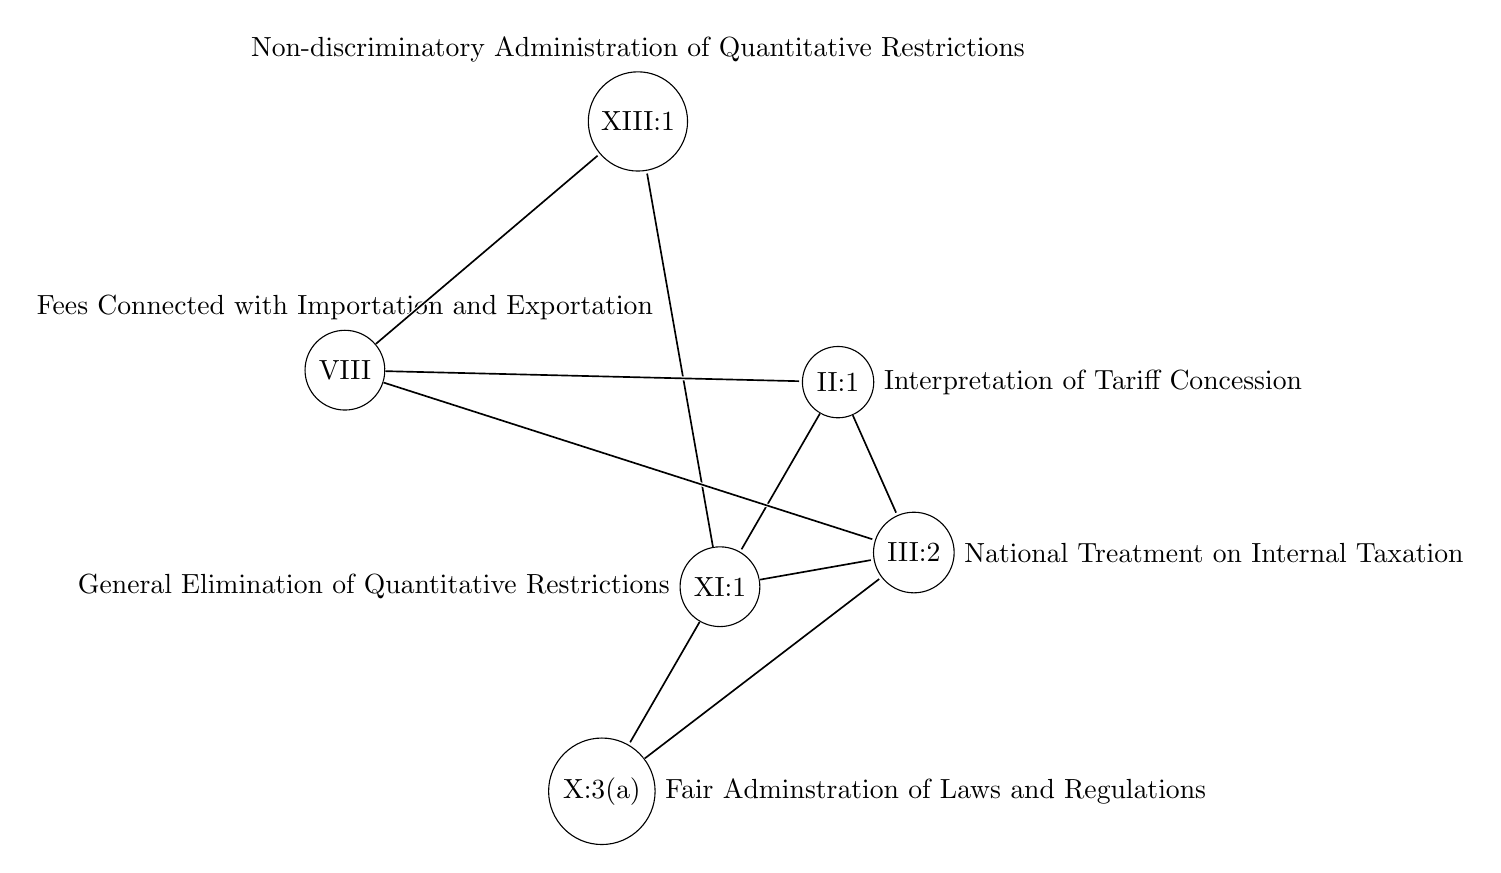
\begin{tikzpicture}[>={Stealth[color=black]},shorten >=1pt,node distance=2cm,on grid,initial/.style={}]
  \node[state, label=right:Interpretation of Tariff Concession] (T1) {II:1};
  \node[state, label=left:General Elimination of Quantitative Restrictions] at ([shift=({240:3 cm})]T1) (T4) {XI:1};
  \node[state, label=right:Fair Adminstration of Laws and Regulations] at ([shift=({240:3 cm})]T4) (T5) {X:3(a)};
  \node[state, label=above:Non-discriminatory Administration of Quantitative Restrictions] at ([shift=({100:6 cm})]T4) (T7) {XIII:1};
  \node[state, label=right:National Treatment on Internal Taxation] at ([shift=({10:2.5 cm})]T4) (T6) {III:2};
  \node[state, label=above:Fees Connected with Importation and Exportation] at ([shift=({150:5.5 cm})]T4) (T8) {VIII};

  \begin{scope}[every edge/.append style={-, double=black, draw=white}] % for directed edge, change "style={->, double=black, draw=white}]"
    \path (T1)
    edge   (T4)
    edge   (T6);
    \path (T4)
    edge   (T5)
    edge   (T6)
    edge   (T7);
    \path (T5)
    edge   (T6);
    \path (T8)
    edge   (T7)
    edge   (T1)
    edge   (T6);

  \end{scope}
\end{tikzpicture}

% to draw the node's border w/ color, refer to https://tex.stackexchange.com/questions/438412/how-to-add-border-to-a-node
  }
  \caption{Market Access}
  \label{fig:f2}
\end{figure}


\section{Conclusion}
I show how WTO works.

\bibliography{bibtemplate}

\section{Appendix}



% == END
\end{document}